\chapter{Material und methodisches Vorgehen}
\textbf{Johanna Hoppe}
\section{Erklärung der Methode}
Ein zentrales Verfahren dieser Arbeit ist die
Immunhistochemie. Dies ist eine histologische Methode, mit der
spezifische Zellstrukturen, beispielsweise Proteine, sichtbar gemacht
werden. Diese Markierung basiert auf der Bindung von Antikörpern an ihre
Zielstruktur und somit auf der Antigen-Antikörper-Reaktion (siehe
Kapitel~2.2). Eine spezielle Form der Immunhistochemie ist die
Immunfluoreszenz mit indirekten Färbungen, welche in den folgenden
Untersuchungen verwendet wird.\footcite{LeicaIHC2026}

Im ersten Schritt der immunhistologischen Färbung wird ein
Primärantikörper auf die Zellstrukturen gegeben. Dieser bindet
spezifisch an das Zielantigen (siehe Abbildung \ref{fig:immnuofMMV}). Dabei unterscheidet man
zwischen polyklonalen und monoklonalen Antikörpern. Polyklonale
Antikörper binden an verschiedene Epitope des Antigens, da sie eine
Mischung mehrerer Antikörper darstellen, während monoklonale Antikörper
spezifisch an ein einzelnes Epitop binden. Sie werden von nur einer
Zelllinie produziert, die auf einen einzigen B-Lymphozyten
zurückgeht.\footcites{DocCheckMonoklonal}{DocCheckIHC}

Im nächsten Schritt bindet der Sekundärantikörper spezifisch an den
verwendeten Primärantikörper. Zudem ist dieser mit einem Farbstoff
gekoppelt, welcher unter dem Fluoreszenzmikroskop farbig sichtbar ist.
Daher spricht man von einem fluoreszenzbasierten Detektionssystem. Durch
den Nachweis des fluoreszierenden Antikörpers können somit die
untersuchten Proteine dargestellt und beispielsweise ihre Lokalisation
untersucht werden (siehe Abbildung \ref{fig:immnuofMMV}).\footcite{DocCheckIHC}
\clearpage
% ── Abbildung 7 ausgelassen ──────────────────────────────────
% Abbildung 7: Prinzip der indirekten Immunfluoreszenz (rechts)
% Quelle: \cite{LeicaMicrosystems2026}
% ─────────────────────────────────────────────────────────────
\begin{figure}[h] % [h] versucht, das Bild hier zu platzieren (hier), [t] für oben, [b] für unten
	\centering % Zentriert das Bild horizontal
	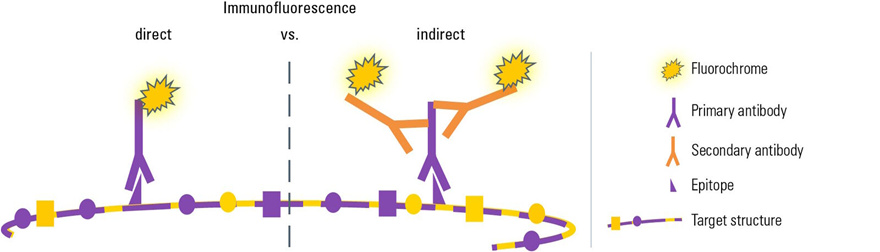
\includegraphics[width=0.91\textwidth]{abbildungen/immunoflurosenzMMV.png} % Lädt das Bild, skaliert es auf 80% der Textbreite
	\caption{ Prinzip der indirekten Immunfluoreszenz (rechts)\parencite{LeicaMicrosystems2026}} % Die Bildunterschrift
	\label{fig:immnuofMMV} % Ein Label für Querverweise (z.B. "siehe Abbildung \ref{fig:beispielbild}")
\end{figure}



Für optimale Färbungsergebnisse ist darauf zu achten, die Fixierung der
Zellen optimal sicherzustellen, geeignete Antikörper sorgfältig
auszuwählen und unspezifische Hintergrundfärbungen zu minimieren.
Letzteres wird unter anderem durch gründliche Waschschritte und
geeignete Blockierungsschritte erreicht. Zudem müssen Negativkontrollen
durchgeführt werden, um unspezifische Bindungen der Antikörper
auszuschließen. Auf diese Weise können die Auswertungen aussagekräftig
und präzise durchgeführt
werden.\footcite{LeicaIHC2026}

Um eine Kolokalisation zweier Proteine bei der mikroskopischen
Auswertung beurteilen zu können, müssen diese in einer Probe durch eine
Doppelfärbung sichtbar gemacht werden. Dazu werden zwei verschiedene,
jeweils proteinspezifische Primärantikörper eingesetzt. Dabei ist zu
beachten, dass diese aus zwei unterschiedlichen Spezies stammen. Die
Sekundärantikörper sind jeweils spezifisch gegen die Spezies des
Primärantikörpers gerichtet, weshalb die Wahl von zwei
unterschiedlichen Spezies die eindeutige Zuordnung der Signale
ermöglicht und Kreuzreaktionen vermeidet. Zudem muss bei einer
Doppelfärbung beachtet werden, dass die an die Sekundärantikörper
gekoppelten Fluoreszenzfarbstoffe sich ausreichend unterscheiden, damit
es zu keiner Überlagerung der Signale kommt. Dies bedeutet, dass die
Spektren, in denen die Farbstoffe fluoreszieren, nicht stark überlappen
dürfen. Diese Spektren ergeben sich aus der jeweiligen Anregungs- und
Emissionswellenlänge.\footcite{Hackenberg}
\section{Begründung der Methodenwahl}
\section{Material}